\section{Feature Learning}
\textbf{Sensitive Sub-Network:} For an input $x\in\R^{d_{in}}$, let $\P^{\S}_{x,t}(\tau_{\S})=\{p\in[P]: |\partial_{\tg} A_t(x,p)|\tau_{\S}\}$ be the set of paths, which have activations whose gradient to any of $\Tg\inrdnet$ is greater than some threshold $\tau>0$. Using the property that the slope of the sigmoid diminishes in the extremities, we note that for appropriate choices of $\tau_{\A}$ (sufficiently close to $1$) and $\tau_{\S}$ (large enough), $\P^{\S}(\tau_{S})\cup \P^{\A}(\tau_{\A})$.
We now take a re-look at the NTF and NTK matrices, and explicitly write down the terms related to feature learning. \hfill\\
$2.$ Let us take the case of classification with cross-entropy loss. Say we have trained till some $T$ epochs with good classification (say close to $100\%$) accuracy. Considering the fact that $\hat{y}_T=\Phi_{\Tg_T}v_{\Theta_T}$, the gradient with respect to $\Tg$ will change the NPF matrix $\Phi_{\Tg_T}$ in such a manner to reduce the loss, i.e., increase the margin of each of the classified examples. We test this hypothesis  of \emph{margin-increase} due to feature learning in the following toy experiment.\hfill\\
\textbf{A Toy Experiment:} We look at a simple neural network with $d_{in}=2$, $w=2$ and $1$-hidden layer (see first diagram on the left in \Cref{fig:feat}). The first layer weights is an identity matrix, and for input $x\in\R^2$ to the network, the first layer output is given by $z_{t}(i)=x(i)G_t(i),i=1,2$, where $G_t(i)=\frac{1}{1+\exp(-\tg(i))},i=1,2$. In this network, there are $2$ paths, and the NPF is given by $\phi_{x,t}=(x(1)G_t(1),x(2)G_t(2))\in \R^2$ (note that this mimics the general structure of the NPF as presented in \Cref{sec:expressivity}).
We check the performance of frozen-gates versus adaptable gates in this network. The dataset is $(x_s,y_s)_{s=1}^{n},n=1000$, wherein, for $s=,1,\ldots,500$, $x_s(1)\stackrel{iid}\sim U[0.1,1]$, and $x_s(2)\stackrel{iid}\sim U[-100,100]$, and $y_s=1$, and for $s=501,\ldots,1000$, $x_s(1)\stackrel{iid}\sim U[-0.1,-1]$, and $x_s(2)\stackrel{iid}\sim U[-100,100]$, and $y_s=-1$. We use the loss function $L_t=\frac{1}{n}\sum_{s=1}^n\frac{1}{1+exp(-y_s\hat{y}_t(x_s))}$. The maximum margin classifier in this case is: predict $+1$ if $x(1)>0$ and else predict $-1$. We trained the simple neural network using gradient descent with step-size of $0.1$, and initialisation $\Tg_0=\Theta_0=(0,0)\in\R^2$ for the following two cases: i) frozen-gates, wherein, we set $\Tg_0=\Tg_t=\Tg_0,\forall t\geq 0$, so that the input features are not transformed, and train only $\Theta_t$ ii) adaptable gates, wherein, we train both $\Tg_t$ and $\Theta_t$. While both cases train for $T=10^4$ epochs, for $T=10^3$ epochs only the model with adaptable gates trains successfully. The results are shown in \Cref{fig:feat}, notice that the right most plot shows that in the case when the gates are adapting, they learn to suppress the second co-ordinate (the scale of $\phi_{x_s,T}$ is from $-15$ to $15$ as opposed to $-100$ to $100$ in $x_s$).
\FloatBarrier
\begin{figure}[h]
\begin{minipage}{0.15\columnwidth}
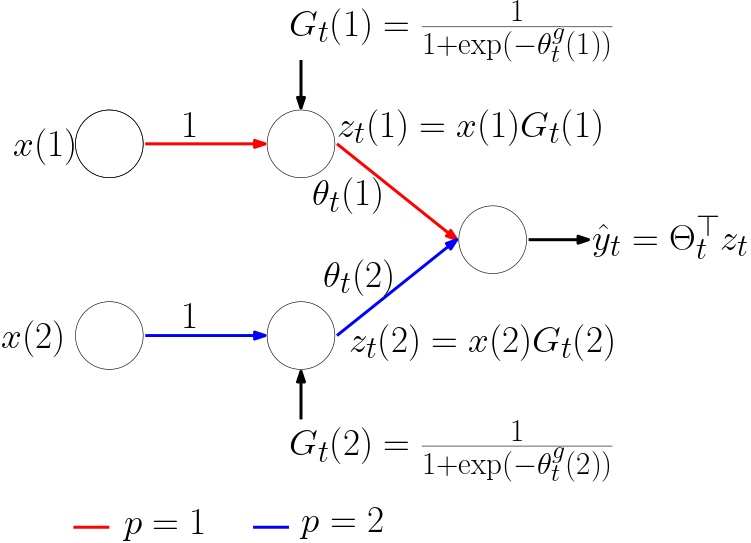
\includegraphics[scale=0.15]{figs/featlearn.png}
\end{minipage}
\hspace{50pt}
\begin{minipage}{0.8\columnwidth}
\resizebox{1\columnwidth}{!}{
\begin{tabular}{cccc}
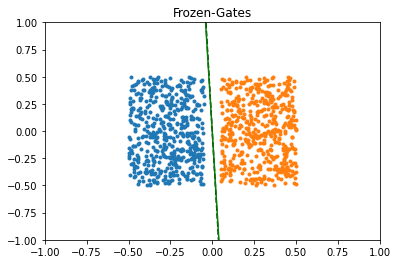
\includegraphics[scale=0.2]{figs/simple-1e2.png}
&
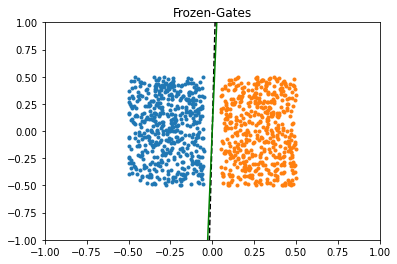
\includegraphics[scale=0.2]{figs/simple-1e3.png}
&
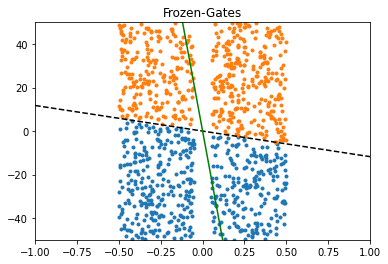
\includegraphics[scale=0.2]{figs/simple.png}
&
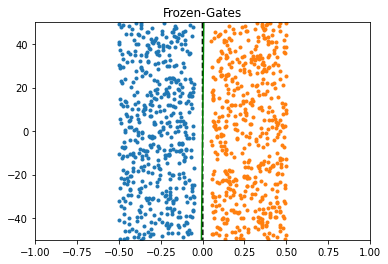
\includegraphics[scale=0.2]{figs/simple-1e4.png}
\\
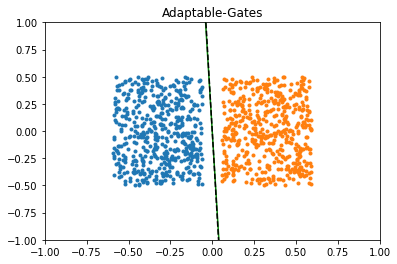
\includegraphics[scale=0.2]{figs/adapt-1e2.png}
&
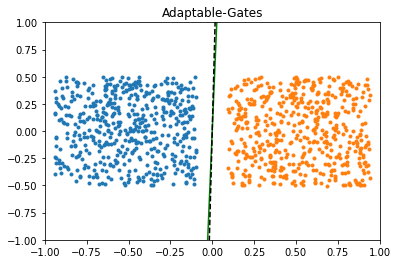
\includegraphics[scale=0.2]{figs/adapt-1e3.png}
&
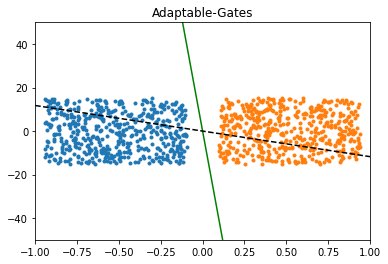
\includegraphics[scale=0.2]{figs/adapt.png}
&
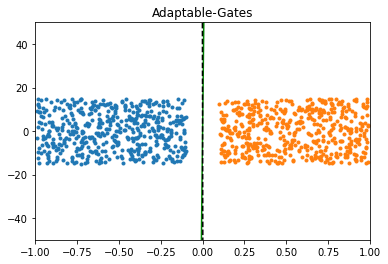
\includegraphics[scale=0.2]{figs/adapt-1e4.png}
\end{tabular}
}
\end{minipage}

\caption{From left: second and third plots shows the training performance of frozen and adaptable gates respectively. In both plots, the bold line in green is the classifier learnt in the case of adaptable gates, and the dotted black line is the classifier learnt in the case of frozen gates. Notice the transformation of the feature space in the case of adaptable gates.}
\label{fig:feat}
\end{figure}
$3.$ \textbf{An open question:} Informally speaking, in the above example, even though the gating parameters had $2$-degrees of freedom, it was nonetheless sufficient to adapt the features. Thus, perhaps we can hypothesise that subject to the `well-conditioned' ness of $K^a_t$, such margin increase can be perhaps achieved for all the $n$ examples.  However, in practice, both $\Tg_t$ as well as $\Theta_t$ change, and an open question is to understand how the joint optimisation and feature learning happens. 